\chapter{Literature Review}
\label{ch:review}
Since 1970s, a great progress has been made in the computer based face recognition area. Face recognition has attracted the attention of researchers from various areas. In this chapter, a literature review on face recognition is present. Because the focus of this research is 2-D face recognition, 3-D face recognition is excluded from the chapter. Most recent approaches for face recognition can be divided into two categories: appearance-based face recognition and model-based face recognition. The appearance-based approaches process face images based on statistical analysis of pixel value distributions. The model-based approaches match a general 2-D face model on face images. Furthermore, a $2.5$D approach - 3-D morphable face model is introduced, which adopts a 3-D face model to extract face representations from 2-D face images. 

The chapter is organised as: \mbox{Section} \ref{sec:appearancebased} introduces appearance-based face recognition; \mbox{Section} \ref{sec:modelbased} describes model-based face recognition; \mbox{Section} \ref{sec:3DMM} gives a brief description of 3-D morphable face model; \mbox{Section} \ref{sec:others} briefly introduces rest major approaches. Some popularly used face databases are presented in \mbox{Section} \ref{sec:facedatabase}.

\section{Appearance-Based Face Recognition}
\label{sec:appearancebased}
Many approaches for object recognition are directly applied on 2-D images. A 2-D face image is treated as a high-dimensional vector. They are so called appearance based approaches. Image data can be represented as vectors which are points in a high dimensional vector space. For example, a $128 \times 128$ image can be represented by a vector $x \in \mathcal{R}^{16384}$. In the high-dimensional space, every object is described if it can be depicted in the $128 \times 128$ image. If all vectors in the high dimensional space are the same type of objects, \textit{e.g.}, faces, the natural constraints of the physical world indicate that the vectors will in fact lie in a lower dimensional linear subspace or non-linear manifold. Linear subspace analysis has significantly advanced facial recognition technology, but it does not have sufficient modelling capacity to preserve the variations of the face manifold and distinguish between different persons to achieve high accuracy in face recognition. Recent developments in nonlinear manifold analysis provide more flexibility and modelling capacity to analyse face manifolds. However, the generalisation of nonlinear methods is affected by the number of examples, \textit{e.g.}, there is a small number of face example images in training set, but large variations of facial appearance during the testing. The phenomenon leads incorrect results and overfitting \cite{Zhao2003}.
\subsection{Linear Analysis}
Three classical linear approaches are introduced here, which are Principal Component Analysis (PCA) \cite{Turk1991}, Independent Component Analysis (ICA) \cite{Bartlett1998} and Linear Discriminant Analysis (LDA) \cite{Belhumeur1997,Swet1996}. By projecting a face image to a subspace, the projection coefficients are used as the feature representation of each face image. The classification is performed between the test face image and the training prototype. All representations from these three linear approaches are considered as a linear transformation from the original image vector $x$ to a projection feature vector $y$, \textit{i.e.},
\begin{equation}
 y = W^T x
\end{equation}
where $W$ indicates the transformation.
\subsubsection{PCA}
Principal Component Analysis (PCA) is to find a subspace which accounts for the distribution of face images within the entire image space. The PCA is generated from the Karhunen-Loeve (KL) expansion, which has been widely used for face representation \cite{Kirby1990} and face recognition \cite{Turk1991}. In \cite{Turk1991}, all face images in the training set are collected and composed into a covariance matrix. The eigenvectors and corresponding eigenvalues are generated from the covariance matrix. The eigenvectors are visualised into a two-dimensional array and display ghost face like appearance. Hence, the eigenvectors are also named ``eigenfaces'' as shown in \mbox{Figure} \ref{fig:eigenfacesreview}.
\begin{figure}[ht]
\begin{center}
 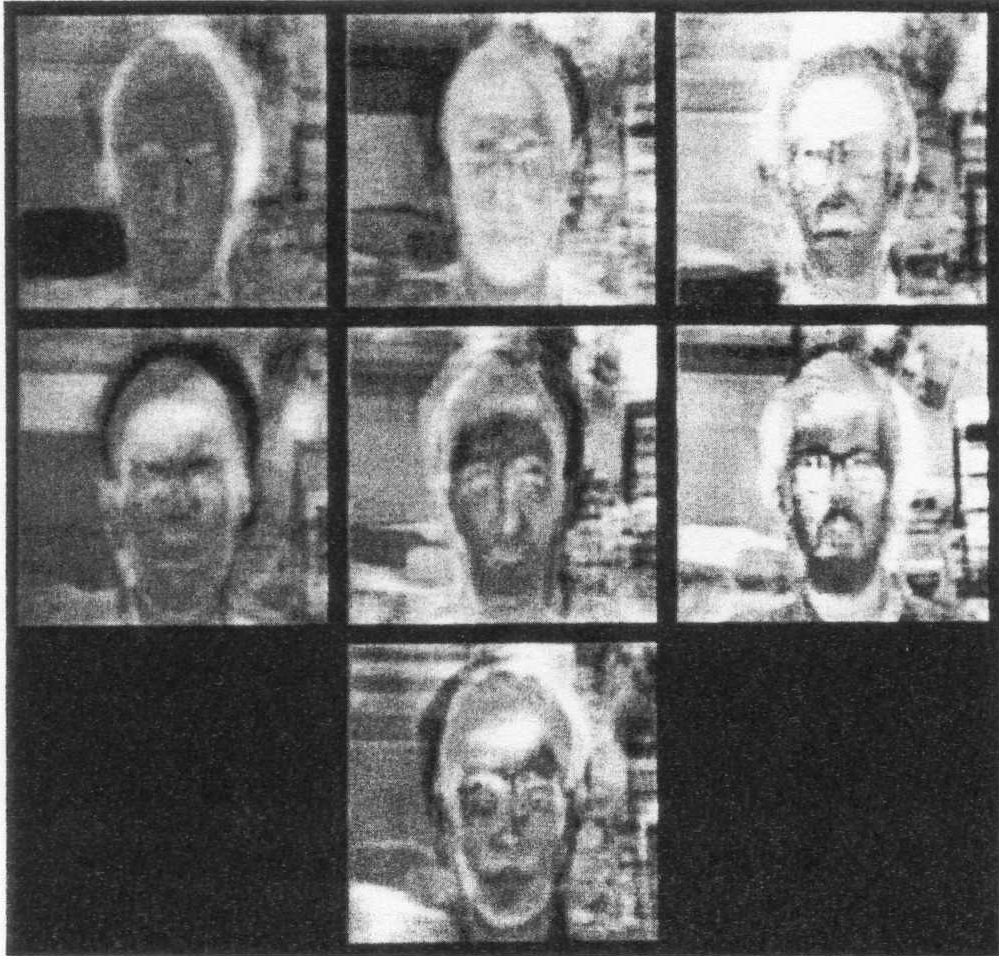
\includegraphics[width=0.8\columnwidth]{ch2/figures/seveneigenfaces.jpg}
\caption{The seven eigenfaces calculated from \cite{Turk1991}}
\label{fig:eigenfacesreview}
\end{center}
\end{figure}  
These eigenfaces span a small subspace in the image space. The subspace is called ``face'' subspace. Given the eigenfaces, every face in the training set can be represented as a vector with a sequence of weights. The weights are obtained by projecting the images into the face subspace by a inner product operation. The testing image is also represented by its vector. The recognition on the PCA approach is done by measuring the Euclidean distance between the testing vector and the existing face vectors in the face subspace. The method is illustrated in \cite{Turk1991} using a large database of $2500$ face images of $16$ subjects with three head orientations, three scales, and three lighting conditions. 

The PCA approach is enhanced in \cite{Pentland1994} by several extensions. The experiments are carried out in a large-scale face database, which contains $7562$ face images of approximately $3000$ people. The first twenty eigenfaces are introduced from a random $128$ images subset. Annotated information on gender, race, approximate age and facial expression is included in the extended approach. A view-based eigenfaces technique is introduced as modular eigenspace so that face recognition can be performed under various poses. The probabilistic analysis is integrated into the eigenface approach in \cite{Moghaddam1997}. The probability density is estimated in the eigenspace. Two types of density estimation are derived from modelling the eigenspaces: a multivariate Gaussian model and a Mixture Gaussian model. By applying Bayes' theorem, the maximum likelihood estimation is used for face detection and face recognition.

Some experiments are conducted to test the performance of the PCA approaches. It is reported that the approach is fair against the illumination change. In \cite{Belhumeur1997}, it is mentioned that by discarding the three most significant eigenvectors, the variation due to lighting is reduced. %Because the first eigenvectors capture the variation due to lighting, the better clustering on the training data is acquired by ignoring these first eigenvectors.

\subsubsection{ICA}
Like the PCA, Independent Component Analysis (ICA) is also a linear transformation. The PCA is to find the ranked principle components which describe the variation, however the ICA is to find the independent components by maximising the statistical independence between these estimated components. The independence of the components is measured by maximising Non-Gaussian distribution. The popular algorithms to computing ICA include infomax \cite{Bell1995}, FastICA \cite{Hyvarinen1999,Hyvarinen2001}, and JADE \cite{Cardoso1996}.

The ICA is a generalised version of the PCA, and the PCA can be derived as a special case of ICA, as Gaussain component models are used. The difference betwen ICA and PCA is illustrated in \mbox{Figure}.\ref{fig:icaVSpca}.
\begin{figure}[ht]
 \begin{center}
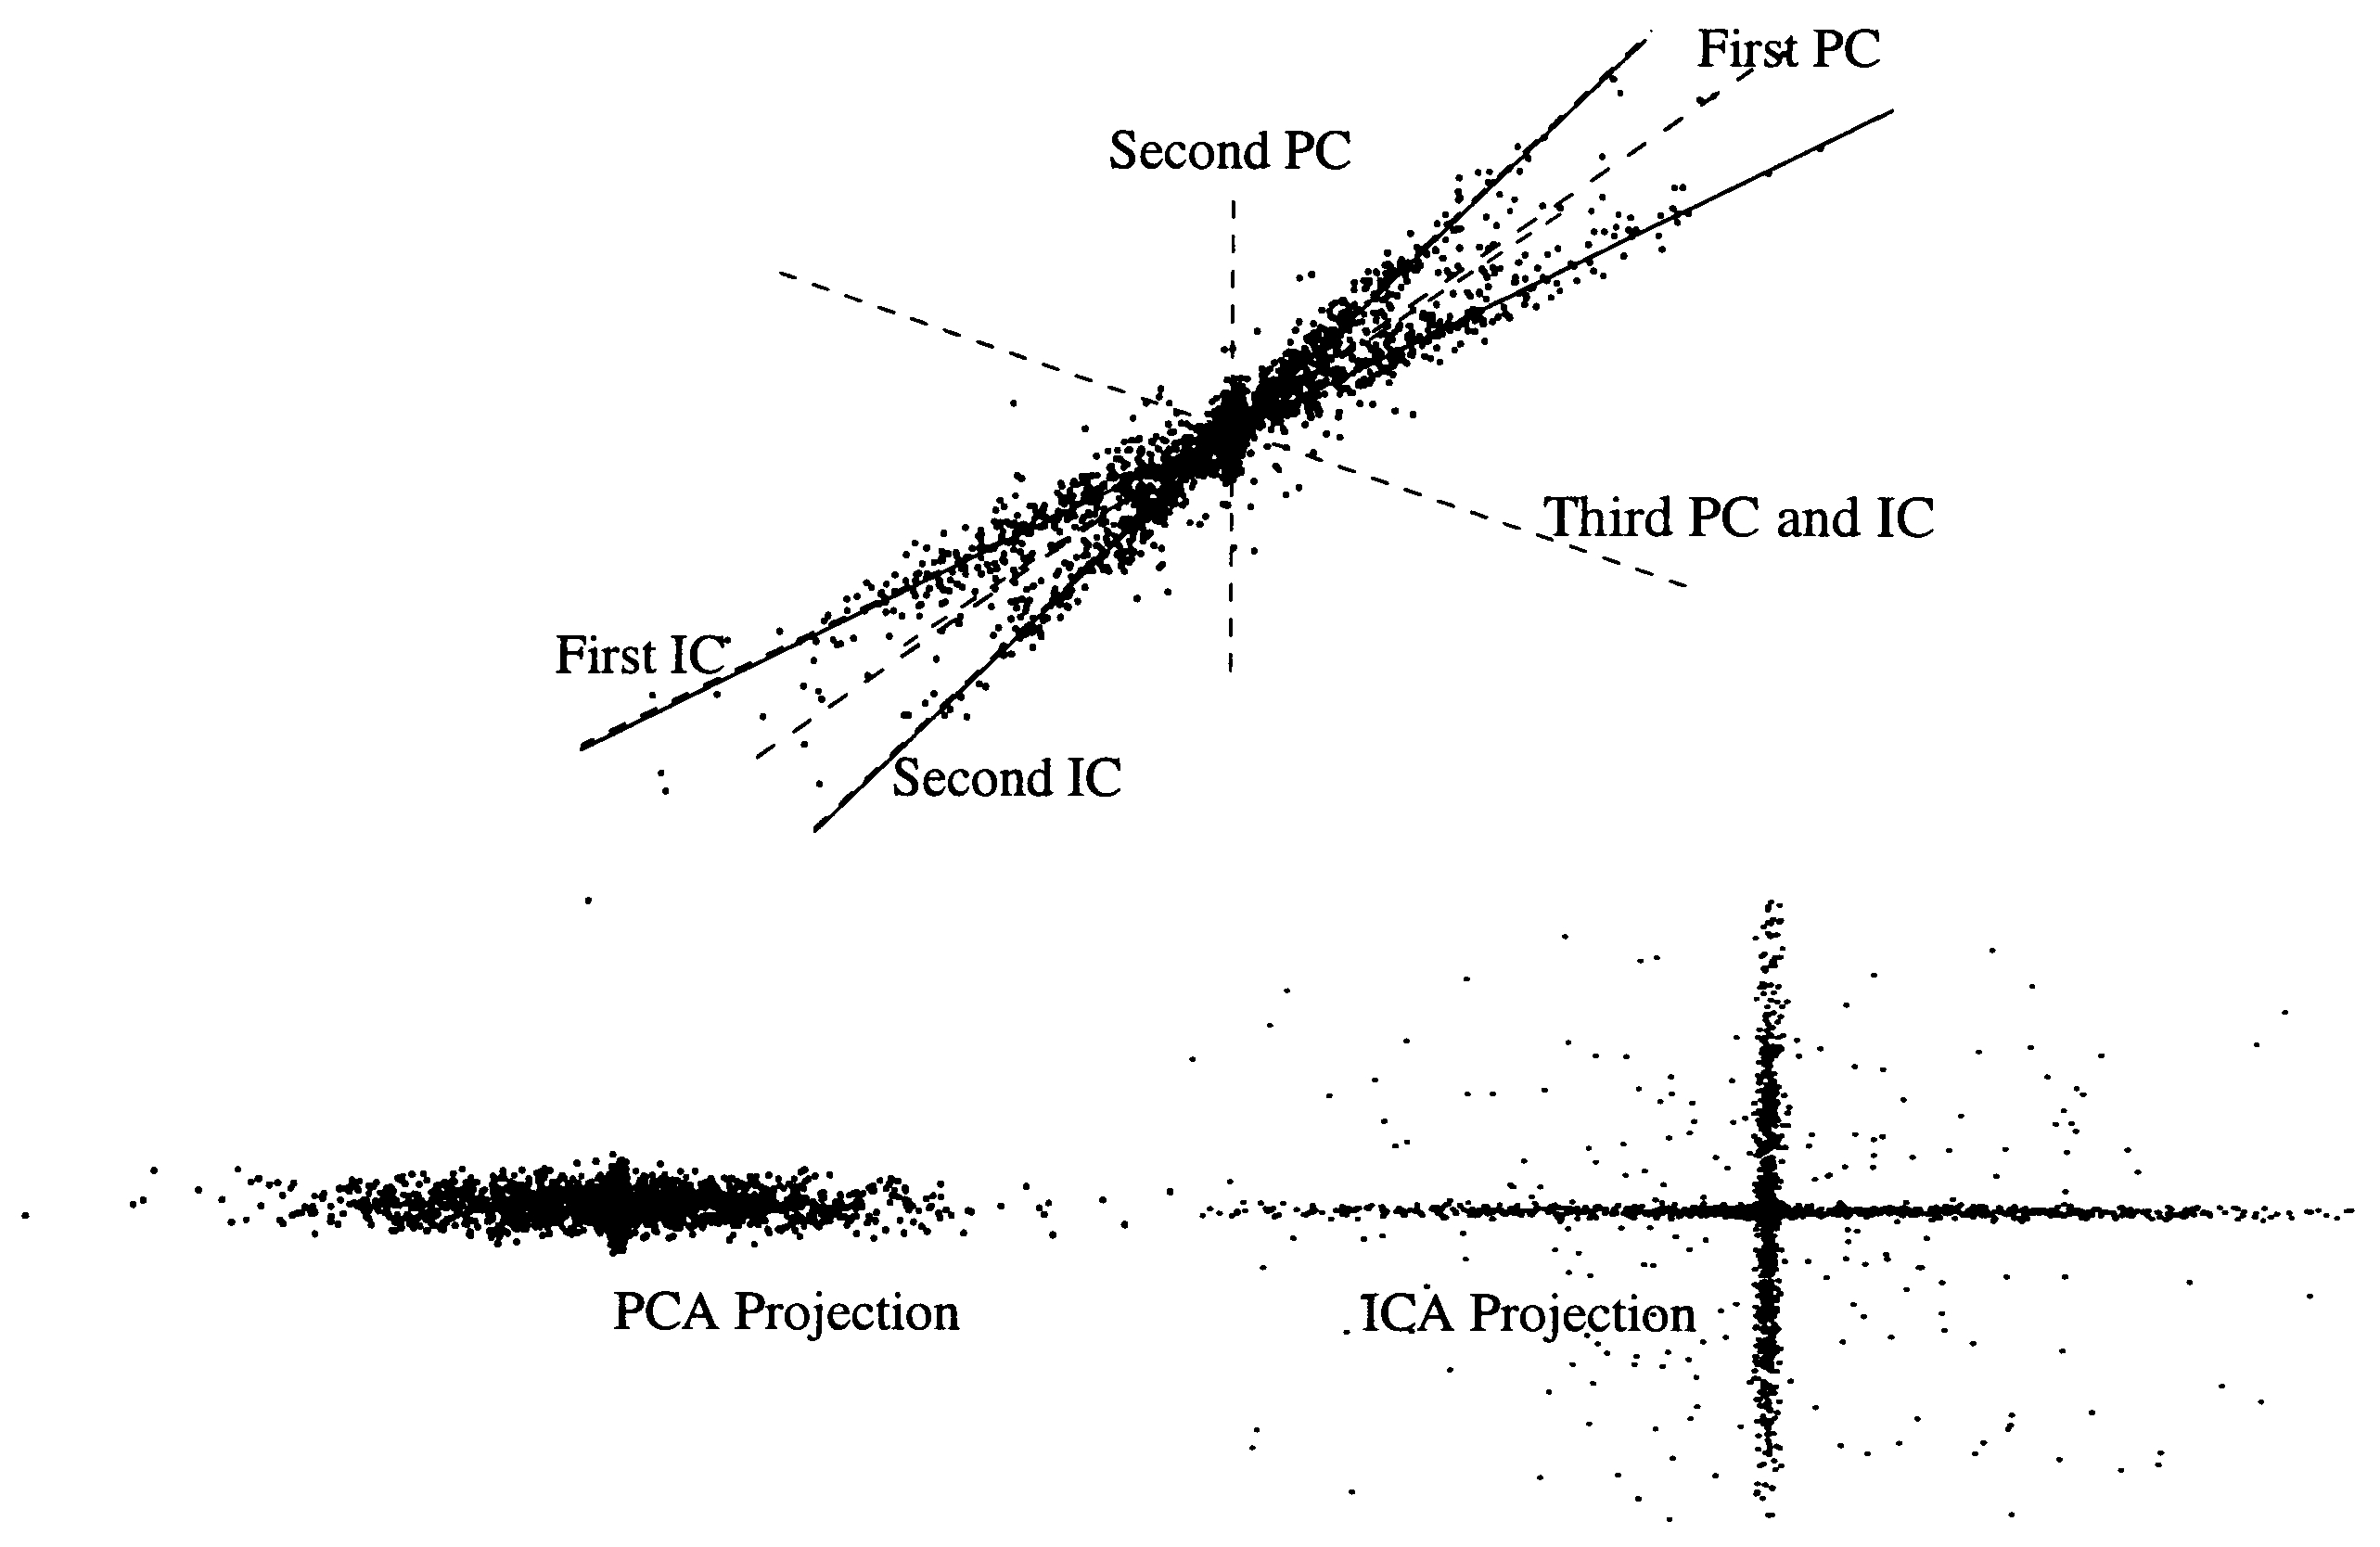
\includegraphics[width=0.7\columnwidth]{ch2/figures/icaVSpca.jpg}
  \caption{The difference between ICA and PCA \cite{Bartlett2002}.}
\label{fig:icaVSpca}
 \end{center}
\end{figure} 
There are 3-D data examples residing in a 3-D axes space. The Independent Component (IC) and Principal Component (PC) construct different coordination systems. The PC axes are orthogonal while the IC axes are not. If only two components are allowed, ICA chooses a different subspace than PCA. In the PCA projection, the data are sparsely distributed on the first PC, but closely clustered on the second PC. In ICA projection, the data are both sparsely distributed on the first and second ICs. Since the ICA axes are nonorthogonal, relative distance between points are different in PCA than in ICA. In \cite{Baek2002}, a comparison between ICA and PCA is given. It shows that the ICA outperforms PCA on a human face recognition task when both using same distance metric, \textit{i.e.}, cosine angle. However, when the L1 norm is adapted, the PCA significantly outperforms ICA.

In \cite{Bartlett2002}, ICA was applied on face recognition in the \mbox{FERET} database under two architectures. In the first architecture, the images are treated as random variables and the pixels are treated as outcome. The spatially local basis images for the faces are found as shown in \mbox{Figure} \ref{fig:25ICs1}.
\begin{figure}[t]
 \begin{center}
  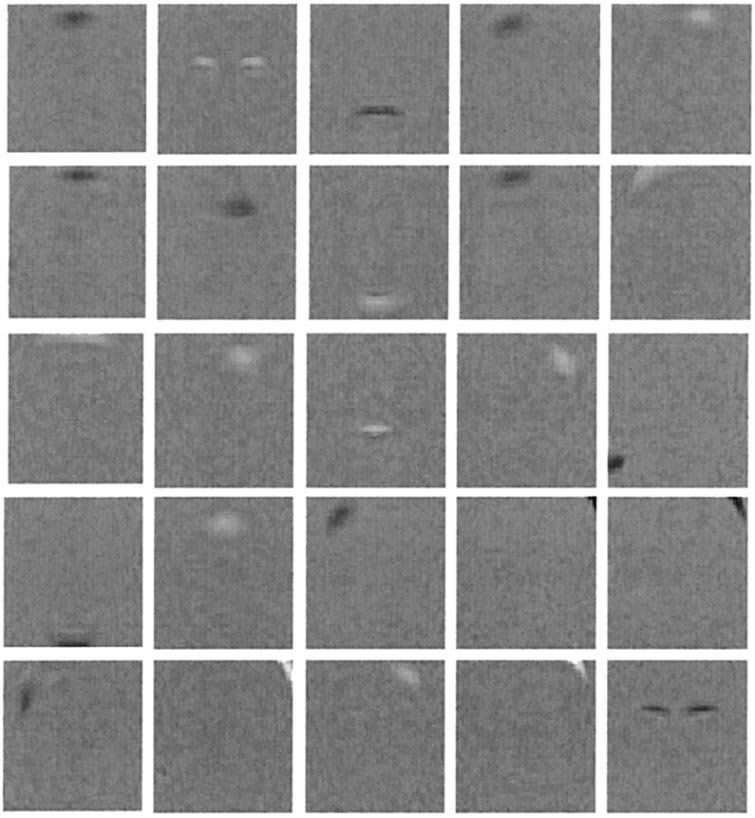
\includegraphics[width=0.7\columnwidth]{ch2/figures/25ICsArch1.jpg}
  \caption{Twenty-five image sets obtained by Architecture I in \cite{Bartlett2002}}
  \label{fig:25ICs1}
 \end{center}
\end{figure} 
In the second architecture, the pixels are treated as random variables, and the images as outcome. A factorial face code is produced in the second architecture. The ICA separates the high-order moments of the input, while the second order moments are utilised in the PCA. The ICA factorial code representation is illustrated in \mbox{Figure} \ref{fig:25ICs2}.
\begin{figure}[ht]
 \begin{center}
  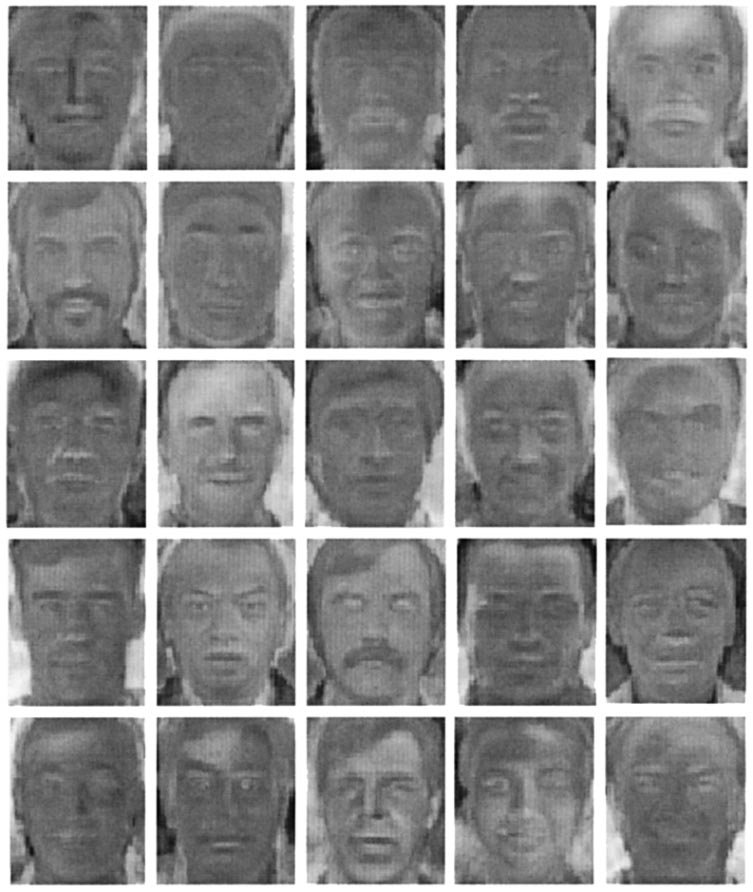
\includegraphics[width=0.7\columnwidth]{ch2/figures/25ICsArch2.jpg}
  \caption{The basis images for the ICA-factorial representation obtained with Architecture II in \cite{Bartlett2002}}
  \label{fig:25ICs2}
 \end{center}
\end{figure} 

Liu and Wechsler \cite{Liu2003} present an independent Gabor feature (IGF) method and its application to face recognition. The method derives independent Gabor features in the feature extraction stage, and an IGF feature-based probabilistic reasoning model (PRM) classification method is developed in the pattern recognition stage. The IGF method is firstly to acquire a Gabor feature vector from a set of Gabor wavelet representations of face images, then to reduce the dimensionality of the vector by means of principal component analysis, and finally to define the independent Gabor features based on the ICA. Experiments on face recognition are carried out by using the FERET and the ORL datasets. The images vary in illumination, expression, pose, and scale. The IGF method achieves $98.5\%$ correct face recognition accuracy when using 180 features for the FERET dataset, and $100\%$ accuracy for the ORL dataset using $88$ features. The approach is extended with enhanced ICA \cite{Liu2004smc}.
\subsubsection{LDA}
Both PCA and ICA are unsupervised methods that yield a set of linear features of a particular dimension, but there is no consideration if this set of features is good for classification. In the PCA, the examples' cluster is maximised not only between different class clusters but also within the same class cluster. The PCA does not take classes into account when there are more than one class in a dataset. This leads to significant problems. For the data set on \mbox{Figure} \ref{fig:PCAbada}, one class is indicated by circles and the other by stars. 
\begin{figure}[ht]
 \begin{center}
  %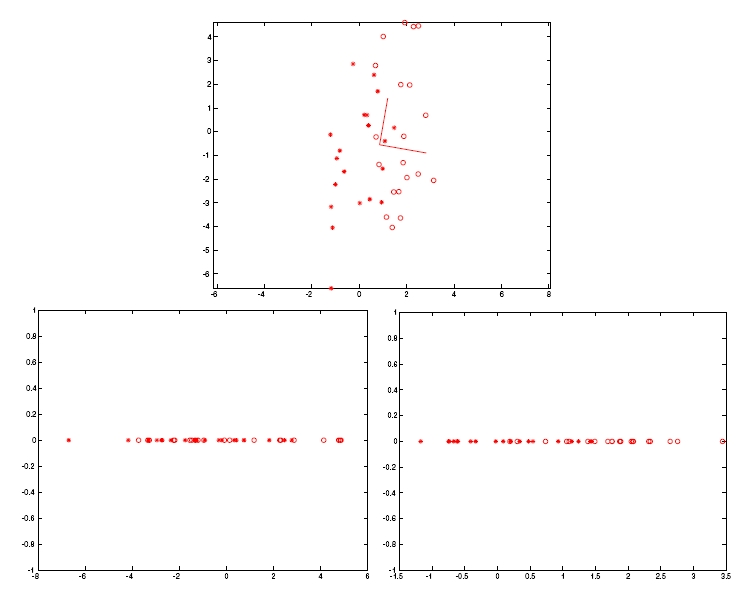
\includegraphics[width=\columnwidth]{ch2/figures/LDAvsPCA.jpg}
  \subfigure[The original 2D data set contains two classes]{\label{fig:PCAbada}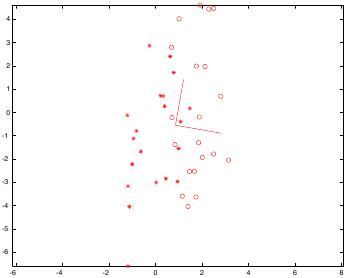
\includegraphics[width=0.45\columnwidth]{ch2/figures/LDAvsPCA_a.jpg}}\\
  \subfigure[The data are projected onto the first PC.]{\label{fig:PCAbadb}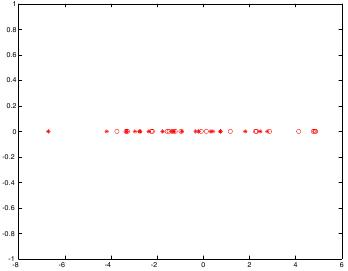
\includegraphics[width=0.45\columnwidth]{ch2/figures/LDAvsPCA_b.jpg}}
  \subfigure[The data are projected onto the second PC.]{\label{fig:PCAbadc}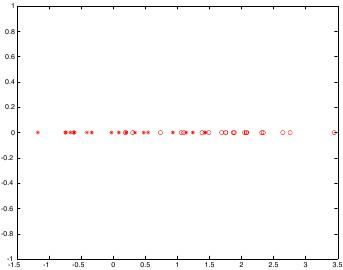
\includegraphics[width=0.45\columnwidth]{ch2/figures/LDAvsPCA_c.jpg}}
 \end{center}
\caption{The PCA has no consideration for classification purpose. \cite{Forsyth2003}}
\label{fig:PCAbad}
\end{figure} 

The PCA would suggest projection onto a vertical axis, which captures the variance in the dataset, but cannot be used to discriminate it from the axes obtained by PCA, which are overlaid on the data set. The bottom of \mbox{Figure} \ref{fig:PCAbad} shows the projections onto those two axes. \mbox{Figure} \ref{fig:PCAbadb} is the projection onto the first PC, which has higher variance, but separates the classes poorly. \mbox{Figure} \ref{fig:PCAbadc} shows the projection onto the second PC, which has significantly lower variance and gives better separation. \mbox{Figure} \ref{fig:PCAbad} shows the first PC would produce a bad classification, while the second PC would produce a good classification, despite the factor that the second PC does not scatter the data.

Linear Discriminant Analysis (LDA) is a statistical method to classify examples into different classes based on a set of measurements of examples. The LDA applied in face recognition is very successful, because LDA is originally for classification, \textit{i.e.}, the LDA is a supervised learning approach. In LDA, the purpose is to maximise the discrimination between different classes, and recognition can be apparently done based on this. The LDA also constructs a subspace that is constructed by the selected components. The LDA training is carried out by using scatter matrices. The method selects a set of features in such a way that the ratio of the between-class scatter and the within-class scatter is maximised. The between-class scatter matrix is defined as
\begin{equation}
 S_B = \sum_{i=1}^c N_i (\mu_i-\mu)(\mu_i-\mu)^T
\end{equation}
and the within-class scatter matrix is defined as
\begin{equation}
 S_W = \sum_{i=1}^c \sum_{x_k \in X_i} (x_k-\mu_i) (x_k - \mu_i)^T
\end{equation}
where $\mu_i$ is the mean image of class $X_i$, and $N_i$ is the number of examples in class $X_i$, and $c$ is the number of classes. If the scatter matrix $S_W$ is nonsingular, the optimal projection $W_{opt}$ is chosen as the matrix with orthonormal columns which maximises the ratio of determinant of the between-class scatter matrix of the projected examples to the determinant of the within-class scatter matrix of the projected examples,\textit{ i.e.}
\begin{equation}
 W_{opt} = \arg \max_W \frac{|W^T S_B W|}{|W^T S_W W|}
\end{equation}
and the projection $W_{opt}$ can expressed as
\begin{equation}
 W_{opt} = [w_1\quad w_2 \quad \ldots \quad w_m]
\end{equation}
where $\{w_i|i=1,2,\ldots,m\}$ is a set of generalised eigenvectors of $S_B$ and $S_W$ corresponding to the $m$ largest generalised eigenvalues. Because an upper bound on $m$ is $c-1$, there are $c-1$ nonzero components.

However, in some real applications, the number of images in the training set $N$ is normally much smaller than the number of pixels in each image $n$, so that the within-class scatter matrix $S_W$ tends to be always singular. The phenomenon is called \textit{small sample size} problem \cite{Fukunaga1990}. 

To overcome the small sample size problem, different methods have been proposed in face recognition literature. 

Some methods reduce the dimension of the original sample space, which has been demonstrated to contain considerable discriminative information. In \cite{Belhumeur1997}, a method called ``Fisherfaces'' is proposed. The method is achieved by using PCA to reduce the dimension of feature space to $N-c$, and then apply the LDA to reduce the dimension further to $c-1$.  In \cite{Zhao1998}, the images are firstly preprocessed by photometrical and geometrical techniques, secondly projected by PCA, then projected by LDA, and finally using Euclidean metric and weight mechanism to make decision. These traditional solutions to the small sample size problem require the incorporation of a PCA step into the LDA framework. PCA is used as a preprocessing step for dimensionality reduction so as to discard the null space of the within-class scatter matrix $S_W$ of the training data set, and then LDA is performed in the lower dimensional PCA subspace.

The PCA+LDA methods discard a null space of the within-class scatter matrix $S_W$, and the null space may contain significant discriminative information. In \cite{Chen2000}, an LDA-based method that makes use of the null space of $S_W$ is proposed. All the examples are firstly projected onto the null space of $S_W$, where the within-class scatter is zero, and then the optimal discriminant vectors of LDA are those vectors that can maximise the between-class scatter. Examples are processed directly in the original high-dimensional input space avoiding the loss of significant discriminatory information. Hence, the approach is called Direct LDA (D-LDA) or Null-space LDA. Various approaches \cite{Huang2002,Lu2003,Wu2004,Cevikalp2004,Fan2004} are developed based on D-LDA and are endeavoured to model and calculate the null space. The main drawback of these approaches is that the computational complexity of determining the null space $S_W$ is very high due to the high dimension in $S_W$ itself.

In \cite{Belhumeur1997}, there is a comparative performance analysis carried out on four methods, which are a correlation-based method, a variant of the linear subspace method \cite{Shashua1994}, a PCA method, and a LDA method. The four methods are tested on the Harvard database \cite{Hallinan1995} and the Yale database \cite{Georghiades2001}. The conclusions are drawn such as
\begin{enumerate}
 \item All linear methods perform well if images in training set are similar to images in testing set.
 \item The LDA method appears to be the best at extrapolating and interpolating over illuminant changing.
 \item The largest three principal components does not improve the performance of the PCA method, so that removing these components can gain the performance.
 \item The best number of selected principal components (PCs) is about $45$.\footnote{the conclusion is corresponding to the experiment in \mbox{Appendix} \ref{apx:pcaca} where the best number is $49$ very close to $45$.} The performance drops, when more than $45$ components are used, 
 \item The LDA method appears to be the best on illuminance changing, but suffers when confronted with various facial expression.
\end{enumerate}

Recently, some progress has been made on linear subspace approaches. In two-dimensional PCA \cite{Yang2004}, an image is represented as a 2-D matrix instead of as a vector, and a two-dimensional PCA algorithm for face recognition is developed. Similar to two-dimensional PCA, Kong \textit{et al.} \cite{Kong2005} generalised the conventional LDA into 2-D Fisher discriminant analysis and applied it to face recognition.

\subsubsection{Summary on linear approaches}
In PCA, the eigenface coefficients in face representation are the most descriptive among the three major linear approaches. Due to many established algorithms or source codes, the PCA is easy to be implemented, and also servers as a baseline algorithm in face recognition. However, the PCA is not discriminative for class separation, since it does not take any class information into account. The ICA utilises higher-order statistics in the training data instead of only the second-order statistics in PCA, but there is no general closed-form solution in ICA. In addition, iterative methods, which are used to obtain the ICA representation, cause large amount of computational time. The LDA utilises the class information in the derivation of the representation for the face recognition task, and is a classification problem instead of subspace represetnation problem. The recognition rate in LDA is the highest among the three major linear approaches. However, due to the small sample size problem, the within-class scatter matrix becomes singular, which leads to poor performance on LDA. In \mbox{Appendix} \ref{apx:pcaca}, the experiment of PCA and Canonical Variate is presented, which is also corresponding to the findings in the chapter. 


\subsection{Non-linear Analysis}
In non-linear analysis, it is assumed that objects reside in non-linear structures. The non-linear structures are normally described as \textit{manifold}. A manifold is an abstract mathematical space in which every point has a neighbourhood which resembles an Euclidean space, but in which the global structure may be more complicated. In a one-dimensional manifold (or one-manifold), every point has a neighbourhood that looks like a segment of a line. Examples of one-manifolds include a line, a circle, and two separate circles. In a two-dimensional manifold, every point has a neighbourhood that looks like a disk. Examples include a plane, the surface of a sphere, and the surface of a torus. Manifolds are important objects in mathematics and physics because they allow more complicated structures to be expressed and understood in terms of the relatively well-understood properties of simpler spaces.

The face manifold is more complicated than that in linear subspace models. Linear subspace approaches approximate the non-linear manifold in a linear way. Therefore, non-linear manifold modelling is directly investigated to find the corresponding non-linear manifold. The comparison between linear approach and non-linear approach is given in \mbox{Figure} \ref{fig:linearvsnon-linear}.
\begin{figure}[ht]
\begin{center}
 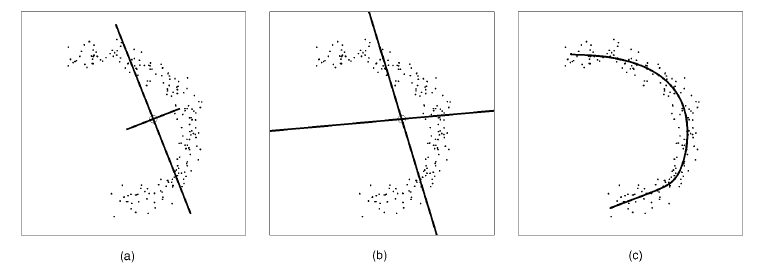
\includegraphics[width=\columnwidth]{ch2/figures/linearvsnonlinear.jpg}
\caption{(a) PCA basis (linear, ordered, and orthogonal). (b) ICA basis (linear, unordered, and nonorthogonal). (c) Principal Curve (parameterised nonlinear manifold). \cite{Moghaddam2002}}
\label{fig:linearvsnon-linear}
\end{center}
\end{figure} 
In \mbox{Figure} \ref{fig:linearvsnon-linear}(a), the principal component vectors are obtained with a toy data set corresponding to an essentially one-dimensional manifold. The first and second components are orthogonal to each other. In \mbox{Figure} \ref{fig:linearvsnon-linear}(b), the ICA produces two unordered nonorthogonal components, one of which is roughly aligned with the first principal component. \mbox{Figure} \ref{fig:linearvsnon-linear}(c) is an example of a principal curve, which is the simplest methods for principal manifold. The principal curve yields a compact and relatively accurate representation of the toy data. Also it displays that for capturing the non-linear manifold, non-linear approach is superior to linear subspace approach.

The classical non-linear approaches such as Kernel PCA \cite{Scholkopf1998}, Kernel LDA \cite{Yang2002}, Kernel ICA  \cite{Bach2002} and Isomap embedding \cite{Tenenbaum2000} are introduced in this subsection.
\subsubsection{Kernel PCA}
The kernel PCA (KPCA) \cite{Scholkopf1998} is to apply an non-linear mapping from the input space $\mathcal{R}^N$ to the feature space $\mathcal{R}^L$ by $\Psi(x): \mathcal{R}^N \rightarrow \mathcal{R}^L$, where $L$ is larger than $N$ and possibly infinite. The mapping $\Psi(x)$ is made by the use of kernel functions meeting the Mercer's theorem \cite{Vapnik1995}
\begin{equation}
 k(x_i,x_j)= (\Psi(x_i)\cdot \Psi(x_j)),
\end{equation}
where the kernel function $k(x_i,x_j)$ in the input space corresponds to dot-products in the higher dimensional feature space. Because computing a covariance matrix is based on dot product, PCA in the feature space can be formulated without direct computation of $\Psi(x)$. Assuming that the mean of the projection of the examples in the feature space is equal to zero, the covariance is given by
\begin{equation}
 \Sigma_K = \langle \Psi(x_i) \Psi(x_i)^T  \rangle
\end{equation}
with resulting eigenvector equation $\lambda V= \Sigma_K V$. The eigenvector solutions $V$ exist with coefficients $\{\omega_i\}$ such that $V=\sum_{i=1}^{T}\omega_i \Psi(x_i)$, where $T$ is the total number of training examples. The equivalent eigenvalue problem can be formulated as
\begin{equation}
 T \lambda \omega = K \omega
\end{equation}
where $\omega$ is a set of $\{\omega_i\}$, and $K$ is a $T\times T$ matrix. The KPCA principal components of any input example can be computed with simple kernel computation against the data set. The $n$-th principal component $y_n$ of the example $x$ is given by
\begin{equation}
 y_n = ( V^n \cdot \Psi(x)) = \sum_{i=1}^T \omega_i^n k(x,x_i)
\end{equation}

Moghaddam \cite{Moghaddam2002} extends the KPCA approach with a \textit{maximum a posteriori} (MAP) matching rule using a Bayesian similarity measure derived from dual probabilistic subspaces. In \cite{Zhou2004}, the KPCA application in face recognition is demonstrated and the recognition performance indicates its advantage over other traditional subspace approaches.
\subsubsection{Kernel LDA}
The Kernel Fisher Linear Discriminant (KFLD) \cite{Yang2002} is similar to KPCA. The projected examples are centred in the feature space. The within-class and between-class scatter matrices are denoted by $S_W^{\Psi}$ and $S_B^{\Psi}$, and applying FLD in kernel space. The eigenvalues $\lambda$ and eigenvectors $w^{\Psi}$ of
\begin{equation}
 \lambda S_W^{\Psi} \omega^{\Psi} = S_B^{\Psi} w^{\Psi}
\end{equation}
which can be obtained by
\begin{equation}
 W_{opt}^{\Psi} = \arg \max_{W^{\Psi}} \frac{|(W^{\Psi})^T S_B^{\Psi} W^{\Psi}|}    {|(W^{\Psi})^T S_W^{\Psi} W^{\Psi}|}  
\end{equation}
where $W_{opt}^{\Psi} =[w_1^{\Psi}\quad w_2^{\Psi}\quad \ldots \quad w_m^{\Psi}]$ is the set of generalised eigenvectors corresponding to the $m$ largest generalised eigenvalues.

For given classes $t$ and $u$ and their examples, the kernel function is defined by
\begin{equation}
 (K_{rs})_{tu} = k(x_{tr}, x_{us}) = \Psi(x_{tr})\cdot \Psi(x_{us}) = \Psi(x_{tr})^T \Psi(x_{us})
\end{equation}
Let $K$ be an $m\times m$ matrix, where $K_{tu}$ is a matrix composed of dot product in the feature space $\mathcal{R}^L$.
From the theory of reproducing kernels, any solution $w^{\Psi} \in \mathcal{R}^L$ must lie in the span of all training examples in $\mathcal{R}^L$. The solution is obtained by solving the following equation 
\begin{equation}
 \lambda K K \alpha = K Z K \alpha
\end{equation}
where $Z$ is an $m\times m$ block diagonal matrix.
The $\Psi(x)$ is projected into a lower dimensional space spanned by the eigenvectors $w^{\Psi}$ in a way similar to KPCA. 

In \cite{Yang2002}, KFLD achieves lower error rates than those in PCA, LDA, ICA, KPCA approaches in face recognition.

\subsubsection{Kernel ICA}
The kernel based ICA is proposed by Bach and Jordan \cite{Bach2002}, who use contrast functions based on canonical correlations in a reproducing kernel Hilbert space to develop a new class of ICA algorithm.

\subsubsection{ISOMAP Embedding}
Isometric Feature Mapping (ISOMAP) \cite{Tenenbaum2000} is a global optimal, and asymptotic method in which convergence guarantees the flexibility to learn a broad class of nonlinear manifolds. The approach seeks to preserve the intrinsic geometry of the data, as captured in the geodesic manifold distances between all pairs of data points. The core is to estimate the geodesic distance between far away points, given only input-space distances. For neighboring points, input space distance provides a good approximation to geodesic distance. For faraway points, geodesic distance can be approximated by adding up between neighboring points. These approximations are computed efficiently by finding shortest path in a graph with edges connecting neighboring data points. \mbox{Figure} \ref{fig:ISOMAP}  describes how ISOMAP exploits geodesic paths for nonlinear dimensionality reduction on the ``Swiss roll'' data set.
\begin{figure}[ht]
 \begin{center}
  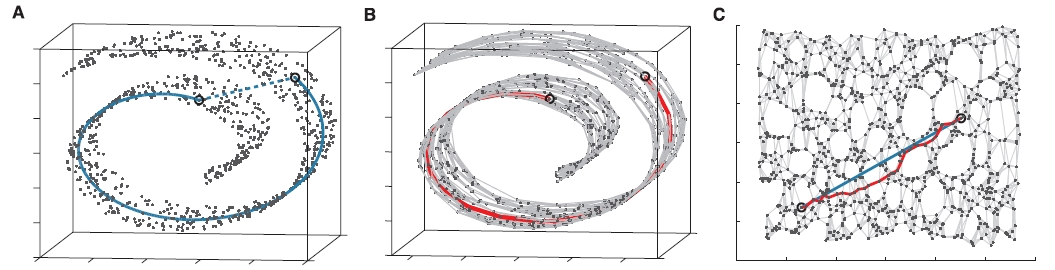
\includegraphics[width=\columnwidth]{ch2/figures/ISOMAP.jpg}
  \caption{ISOMAP exploits geodesic paths on the ``Swiss roll'' data set.}
  \label{fig:ISOMAP}
 \end{center}
\end{figure} 
In \mbox{Figure} \ref{fig:ISOMAP}(A), there are two arbitrary points (circled) on a nonlinear manifold. The Euclidean distance between them in the high dimensional input space may not accurately reflect their intrinsic similarity, as measured by geodesic distance along the low-dimensional manifold (length of solid curve). In \mbox{Figure} \ref{fig:ISOMAP}(B), the neighbourhood graph $G$ constructed in ISOMAP with $k$-near neighour with $k=7$ on $1000$ data points. It allows an approximation (red segments) to the true geodesic path to be computed. \mbox{Figure} \ref{fig:ISOMAP}(C) shows the two-dimensional embedding recovered by ISOMAP, which best preserves the shorest path distances in the neighbourhood graph. Straight lines in the embedding represent simpler and cleaner approximations to the true geodesic paths than do the corresponding graph path (red lines).

Yang \cite{Yang2002ICIP} presents an extended ISOMAP method that utilise LDA for pattern classification, and shows promising results compared with other best classification methods.

\subsection{Bayesian Framework}
In some face recognition systems, a probabilistic similarity between faces is measured based on Bayesian framework. In \cite{Moghaddam1997, Moghaddam2000}, the eigenface method is proposed based on simple subspace norms with a probabilistic model. The similarity between faces on a standard Bayesian analysis of image is divided into two classes: \textit{intra-personal difference} and \textit{extra-personal difference}. The intra-personal difference measures the variations in the appearance of the same person with different expressions and illuminations, while the extra-personal difference measures the variations in the appearance between different persons. The high-dimensional probability density functions for each class are estimated from training data with either single modal density or multimodal densities. The similarity of faces is measured based on \textit{maximise a posteriori }(MAP) probability to decide intra-personal difference or extra-personal difference. In \cite{Moghaddam2000}, Moghaddam \textit{et al.} also proposed an face alignment process (see \mbox{Figure} \ref{fig:facealign}) used in face recognition systems.
\begin{figure}[ht]
 \begin{center}
  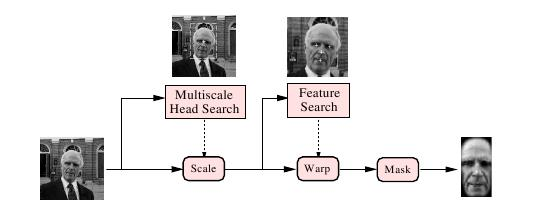
\includegraphics[width=\columnwidth]{ch2/figures/facealignsystem.jpg}
  \caption{The face alignment process \cite{Moghaddam2000}}
  \label{fig:facealign}
 \end{center}
\end{figure} 
\subsection{Summary on appearance-based approaches}
Over the past $30$ years, appearance-based face recognition has been explored and many efficient algorithms have been developed. However, current appearance-based approaches in face recognition systems encounter difficulties in practice due to the small number of available training face images and complex facial variations in the test images. Human face appearance has a number of variations in different lighting conditions, head pose, and facial expressions. There are only small number of images avaliable for training. If a sufficient amount of representative data is not available, a switch \cite{Martinez2001} from non-discriminant techniques to discriminant techniques may lead to poor system performance. Some other techniques, such as face synthesis, can obtain additional training images from the available training data. These techniques \cite{Zhao2000} are helpful to enhance the performance of face recognition. Furthermore, the techniques such as classifier fusion \cite{Lu2003fusion} can help to enhance the performance of face recognition systems.

\section{Model-Based Face Recognition}\label{sec:modelbased}
The model-based approaches in face recognition is to build a model of the human face, which is a flexible model capable to capture facial variations. The prior knowledge of a human face is applied in building up the model, such as the distance between relative feature positions among facial landmarks (i.e. eyes, nose, etc). Early approaches \cite{Galton1888,Bledsoe1964,Kelly1970,Kanade1977} are developed based on localising positions of facial landmarks. A recent feature-based system, \textit{i.e.}, Elastic Bunch Graph Matching \cite{Wiskott1997}, is to find the topological relationship and feature values. Active Shape/Appearance Model \cite{Cootes1996} uses shape and texture information. The model-based approaches usually contain three stages: model construction, model fitting/matching, and recognition.
\subsection{Early Approaches}
The original approach for face recognition can be traced to 1888 by Galton \cite{Galton1888}. A framework for face recognition is proposed by collecting facial profiles. The facial profiles are drawn into curves as shown in \mbox{Figure} \ref{fig:Galton1888}, and the norm of these curves are discovered. The facial profiles are classified by measuring their deviations from the norm.
\begin{figure}[ht]
 \begin{center}
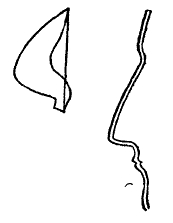
\includegraphics[scale=0.5]{ch2/figures/Galton1888.jpg}
  \caption{The curves depicted from facial profiles \cite{Galton1888}}
\label{fig:Galton1888}
 \end{center}
\end{figure} 

Following the idea, many face recognition systems have been developed in 60s to 70s of 20th century due to the employment of computers. In \cite{Bledsoe1964}, facial feature points are manually located by human operators. The positions of these points are feed to nearest neighbour or other classifiers for identifying the label of the test image. A similar face recognition system without human intervention is developed by Kelly \cite{Kelly1970}. The recognition is determined by measurements of features, \textit{e.g.}, width of head, distance between eyes, distance from top of head to eyes, distance between eyes to nose, and distance from eyes to mouth. In \cite{Kanade1977}, facial feature points are located in two stages: coarse-grain stage and fine-grain stage. The coarse-grain stage simplifies the succeeding differential operation and feature finding algorithms. The fine-grain stage confines the processing to four smaller regions. The two stage processes are depicted in \mbox{Figure} \ref{fig:Kanade1977}. 
\begin{figure}[ht]
  \begin{center}
  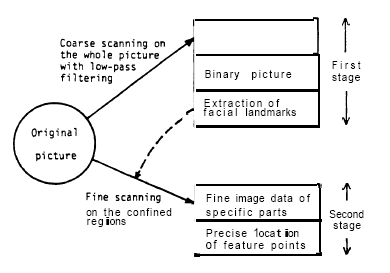
\includegraphics[width=0.8\columnwidth]{ch2/figures/kanade1977.jpg}
   \caption{Two-stage process for computer measurement of features of human-face photographs. \cite{Kanade1977}}
 \label{fig:Kanade1977}
  \end{center}
\end{figure}
 
Human face is characterised by geometrical parameterisation. These parameters may be the distance or angles between key feature points on face images. These methods are limited by storage capacity and computational speed, and are not popular now.

\subsection{Elastic Bunch Graph Matching}
Elastic Bunch Graph Matching (EBGM) is originated from Dynamic Link Architecture (DLA) framework \cite{Lades1993}. The DLA started by computing Gabor wavelets, and then it performs a flexible template comparison between resulting image decompositions using graph-matching. Object recognition is formulated as elastic graph matching, which is operated by loose optimisation of a cost function. \mbox{Figure} \ref{fig:DLA} shows the example of DLA model and graph matching on human faces.
\begin{figure}[ht]
 \begin{center}
  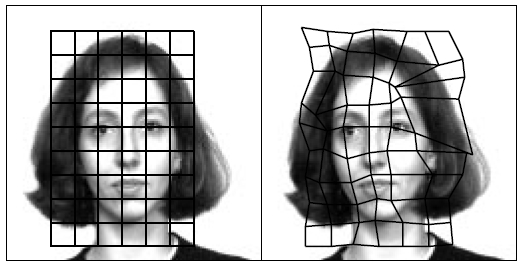
\includegraphics[width=0.77\columnwidth]{ch2/figures/DLAmodel.jpg}
  \caption{The example of DLA model and graph matching.\cite{Lades1993}}
  \label{fig:DLA}
 \end{center}
\end{figure} 
The left part displays the example of a stored object - human face, represented by a rectangular grid form of model graph. The vertices are labeled with magnitude coefficients of Gabor wavelets. The matching begins with an undistorted copy of the object graph. The right part displays the results after grid graph matched with face images. The graph is firstly positioned by ``global moves'', and it is then modified by individual Gabor wavelets diffusion. The grid demonstrates that the graph is accepted as the best match.
\subsubsection{Graphs}
The model of EBGM approach is called \textit{labeled graph}. A labeled graph $\mathcal{G}$ contains $N$ nodes connected by $E$ edges. The nodes are called \textit{fiducial points}, which are facial landmarks, \textit{e.g.}, the pupils, the corners of the mouth, the tip of the nose, the top and bottom of the ears. The graph is object-adapted. If the object is represented by human faces, the geometrical structure is adapted to the structure of human faces as shown in \mbox{Figure} \ref{fig:graphs}.
\begin{figure}[ht]
 \begin{center}
  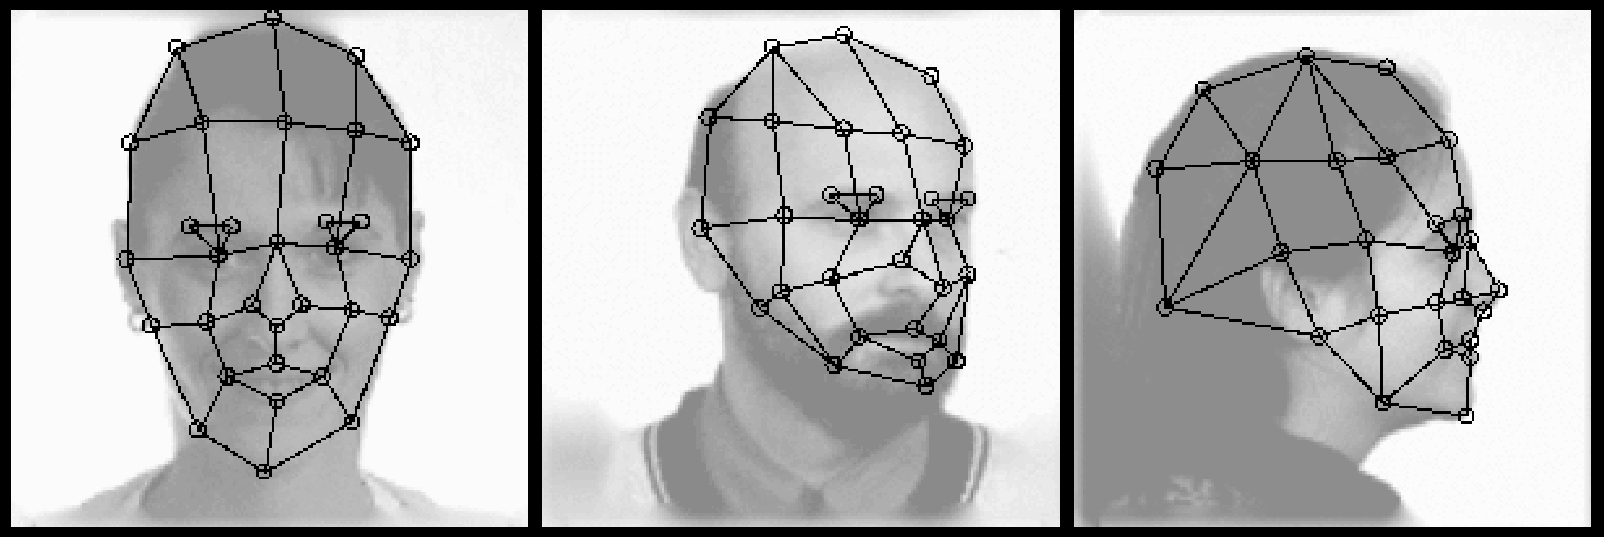
\includegraphics[width=0.77\columnwidth]{ch2/figures/EBGMgrid.jpg}
  \caption{Multiview faces overlaid with labeled graphs. \cite{Wiskott1997}}
  \label{fig:graphs}
 \end{center}
\end{figure} 
There are face-adapted graphs for different poses. These nodes are positioned automatically by elastic bunch graph matching. Each node is also known as a jet. A jet is based on a wavelet transform, defined as a convolution of the image with a family of Gabor kernels. Hence, a jet $J$ is defined as the set of $40$ complex Gabor wavelet coefficients obtained for one image pixel. These $40$ Gabor wavelets are varied with $5$ different spatial frequencies and $8$ orientations. The jet containing the imaginary and magnitude of the coefficients from the convolution is demonstrated in \mbox{Figure} \ref{fig:AGaborJet}.
\begin{figure}[ht]
 \begin{center}
  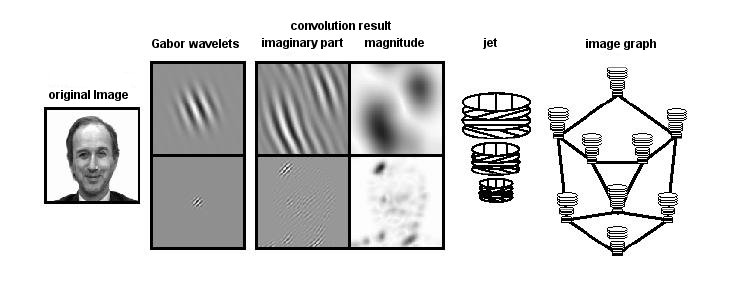
\includegraphics[width=\columnwidth]{ch2/figures/AJet.jpg}
  \caption{The graph representation of a face is based on the jets. \cite{Wiskott1999}}
  \label{fig:AGaborJet}
 \end{center}
\end{figure}  
The graph representation of a face is based on the Gabor wavelet transform, \textit{i.e.}, a convolution with a set of Gabor wavelet kernel. The phase coefficients vary approximately with wavelet frequencies. %For clarity, only 3 frequencies and 4 orientations are represented. 

To extract image graphs automatically, a general representation rather than individual models is needed for face recognition. The representation should cover a wide range of possible variations in the appearance of faces, such as different contoured eyes, mouth, or noses, beards, variations with different gender, age and race, etc. The general representation is in a stack-like structure, which combines a set of $M$ individual model graphs. The combined graph is called a \textit{face bunch graph} (FBG). \mbox{Figure} \ref{fig:FBG} shows the Face Bunch Graph.
\begin{figure}[ht]
 \begin{center}
  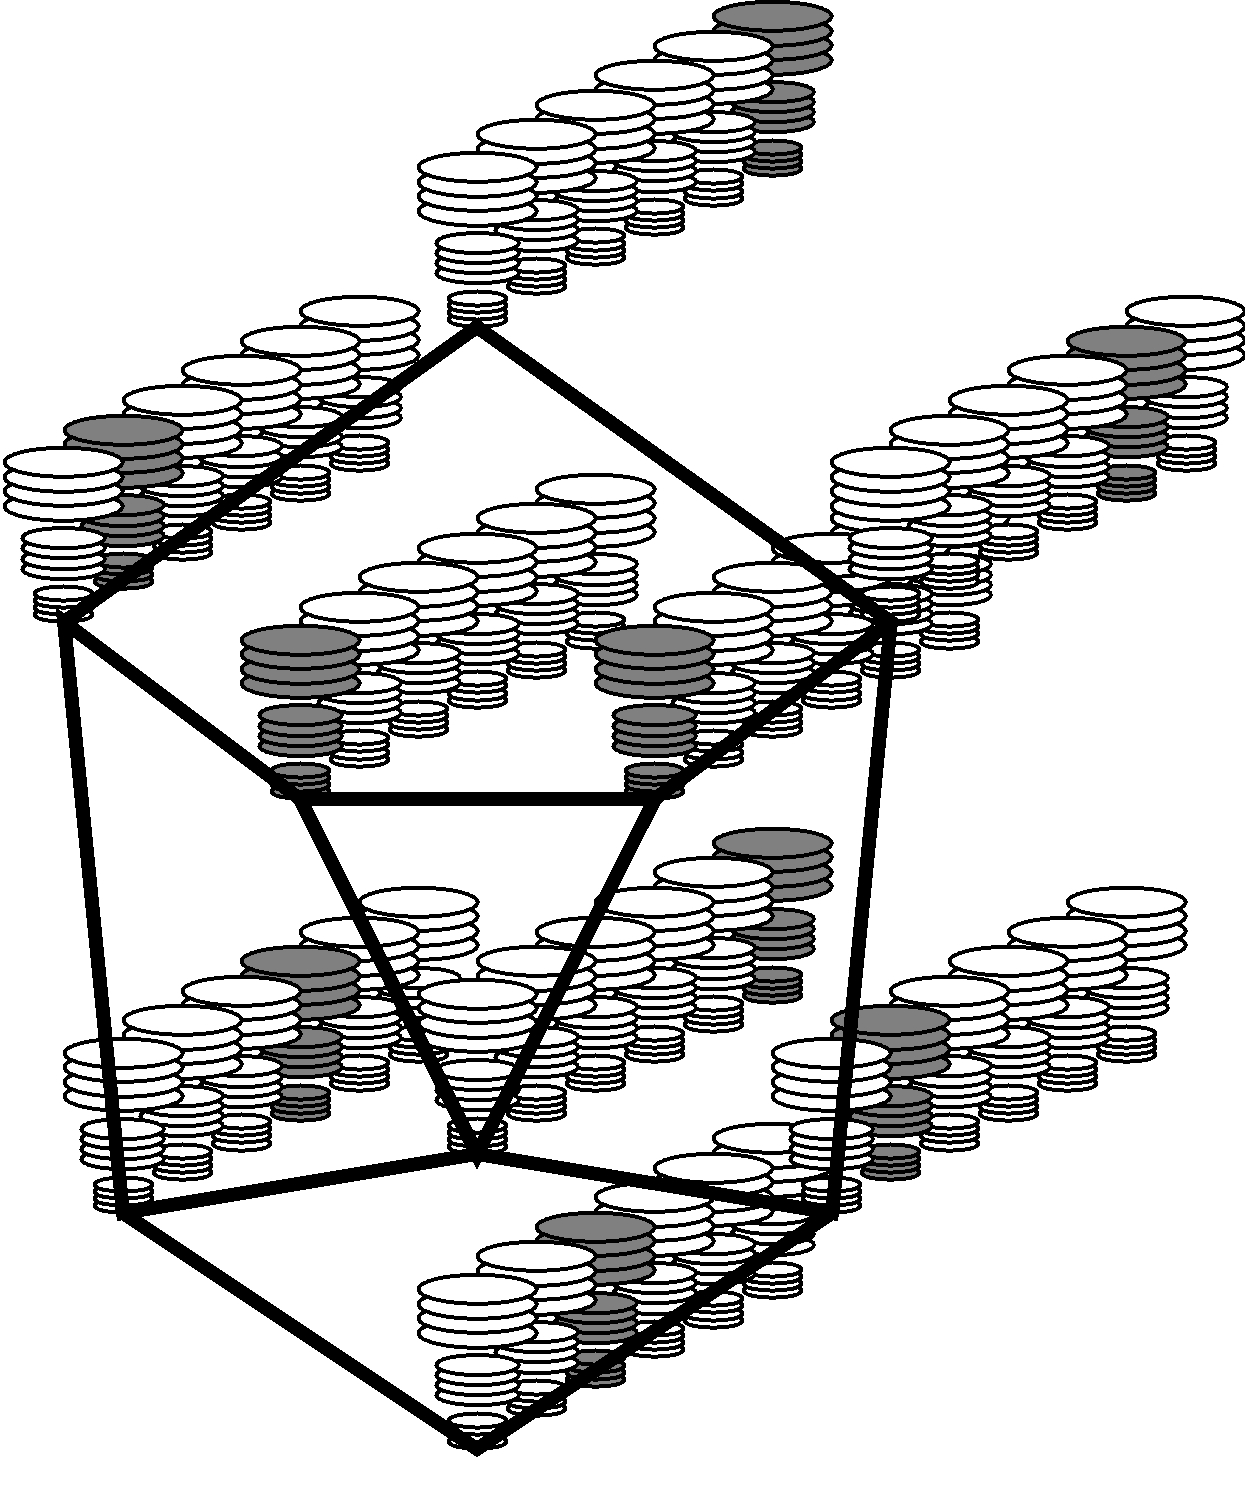
\includegraphics[scale=0.125]{ch2/figures/FBG.jpg}
  \caption{The Face Bunch Graph (FBG) serves as a general representation of faces. \cite{Wiskott1997}}
  \label{fig:FBG}
 \end{center}
\end{figure} 
Each model graph has the same structure. Nodes are referred to identical fiducial points called bunch. An eye bunch containing a set of jets, may represent closed, open, female and male eyes etc. 
\subsubsection{Graph Matching}
To represent a new face, the nodes are positioned on the face image by elastic bunch graph matching. A first set of graph is generated manually by locating fiducial points and connecting edges between them. Once an FBG is well defined, graphs for new images can be automatically generated by elastic bunch graph matching. Matching a FBG with a new image is done by maximising a graph similarity between an image graph and the FBG of identical pose. The graph similarity depends on the similarities of the jets and the topographic structure. Since the FBG provides several jets for every fiducial point, the best jet can be selected and reviewed. A heuristic algorithm is used to find the image which maximises the graph similarity function. The algorithm is as follows:
\begin{enumerate}
 \item The location of the face is found by a sparse scanning of the FBG over image.
 \item The size and position of face are refined. The FBG is varied in size and aspect ratio to adapt the right format of the face.
 \item All nodes are moved locally and relative to each other to optimise the graph similarity.
\end{enumerate}
The coarse to fine approach is applied so that the graph is extracted from the face image.
\subsubsection{Recognition}
After the graph has been generated from a new face image, the face is identified by comparing the similarity between an image graph and all model graphs. The graph with the highest similarity value is selected as the identity. The similarity function is an average over the similarities between pairs of corresponding jets. In \cite{Tefas2001}, the recognition of EBGM is enhanced by an approach using Support Vector Machine (SVM) which addresses the derivation of optimal coefficients. The coefficients measuring the local similarity values are determined by the elastic graph matching procedure at each grid node.

\subsection{Active Appearance Model}
An Active Appearance Model (AAM) is a statistical model generated by combining a model of shape variation with a model of texture variation. In the AAM, ``texture'' means the pattern of grey-level values (intensities) or colours across an image patch. The AAM successfully generalises almost every valid examples, but it brings optimisation difficulties on parameter selection. 
\subsubsection{Shape Models}
Building a shape model is based on a set of annotated face images. In these annotated face images, landmark points on faces are marked manually. These landmarks correspond to the key positions and outline of faces (as shown in \mbox{Figure} \ref{fig:labelled}). The shape is described in $n$ landmark points in 2-D images, so that the shape is represented by a vector $\mathbf{x}=(x_1,\ldots ,x_n,y_1,\ldots,y_n)^T$. In \cite{Edwards1998}, there are $400$ labelled face images , \textit{i.e.}, $400$ different shapes in the face image dataset. To align these shapes into a common coordinate frame, \textit{Procrustes analysis} \cite{Goodall1991} is used to minimise the sum of distances of each shape to the mean. Because the dimensionality of the shape vector $\mathbf{x}$ is high, PCA is used to reduce it into a more manageable manner. The shape vector $\mathbf{x}$ can be approximated through
\begin{equation}
 \mathbf{x} \approx \bar{\mathrm{x}} + \mathbf{\Phi} \mathbf{b}_s
\label{eq:APMPCA}
\end{equation}
where $\mathbf{\Phi}$ contains $t$ eigenvectors corresponding to the first $t$ largest eigenvalues, and $\bar{\mathrm{x}}$ is the mean shape. The vector $\mathbf{b}_s$ defines a set of $t$ parameters of a deformable model. Also \mbox{Equation} \ref{eq:APMPCA} can be formulated in a linear model
\begin{equation}
 \mathbf{x} =\bar{\mathrm{x}} + \mathbf{P}_s \mathbf{b}_s
\end{equation}
where $\mathbf{P}_s$ represents these $t$ eigenvectors, also called a set of orthogonal modes of shape variation. The number $t$ can be chosen so that the deformable model represents a $98\%$ proportion of the total variance of the data. A model of an image is described by the shape parameter $\mathbf{b}_s$, combined with a transformation from the coordinate frame. The parameters for the shape model is $(X_t,Y_t,s,\theta,\mathbf{b}_s)$ where $(X_t,Y_t)$ denotes the translation position, $s$ is the scaling factor, and $\theta$ is the rotation.
 \begin{figure}
  \begin{center}
   \subfigure[Labelled image]{\label{fig:labelled}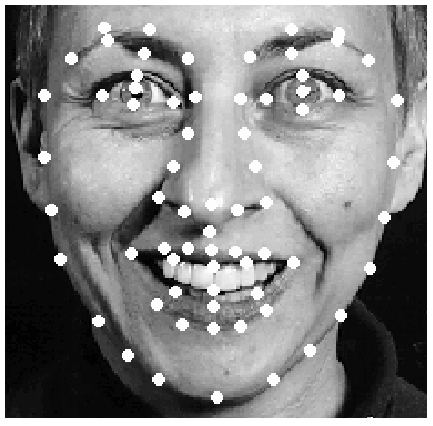
\includegraphics[scale=0.3]{ch2/figures/APMlabelledface.jpg}}
   \subfigure[Points]{\label{fig:points}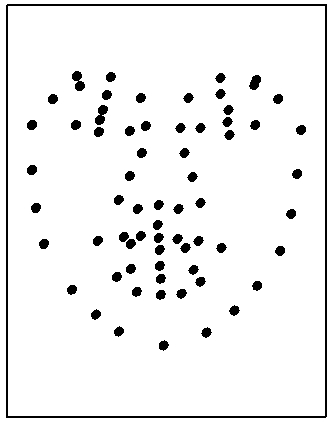
\includegraphics[scale=0.3]{ch2/figures/APMPoints.jpg}}
   \subfigure[Shape-free patch]{\label{fig:patch}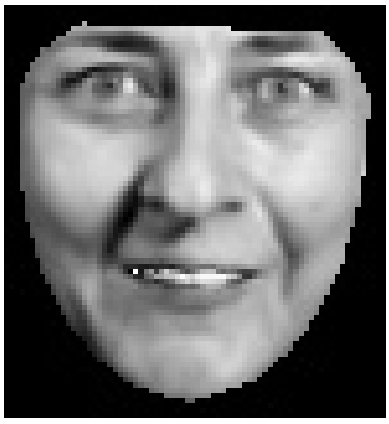
\includegraphics[scale=0.3]{ch2/figures/shapefreepatch.jpg}}
   \caption{A labelled training image gives a set of points and a shape-free patch.\cite{Cootes2001}}
  \end{center}
 \end{figure} 
\subsubsection{Appearance Models}
To build a texture model, \textit{triangulation algorithm} \cite{Cootes2000} is used to warp each example image. The control points on each image are matched against the mean shape model, so that a ``shape-free patch'' is obtained (shown in \mbox{Figure} \ref{fig:patch}). The shape-free patch is represented by a pixel-based grey-level vector $\mathbf{g}$. By applying PCA to the normalised patches generated from the training image set, a linear model is obtained as
\begin{equation}
 \mathbf{g} = \bar{\mathbf{g}} + \mathbf{P}_g \mathbf{b}_g
\end{equation}
where $\bar{\mathbf{g}}$ is the mean normalised grey-level vector, $\mathbf{P}_g$ is a set of orthogonal modes of grey-level variation, \textit{i.e.}, a set of eigenvectors, and $\mathbf{b}_g$ is a set of texture parameters.

The shape and texture of any example can be combined by the parameter vectors $\mathbf{b}_s$ and $\mathbf{b}_g$. The combined appearance model is
\begin{equation}
 \mathbf{b} = \left ( 
		\begin{array}{c}
		 \mathbf{W}_s \mathbf{b}_s \\
		 \mathbf{b}_g
		\end{array}
                   \right ) =
\left ( 
	\begin{array}{c}
	  \mathbf{W}_s \mathbf{P}_s^T(\mathbf{x}-\bar{\mathbf{x}}) \\
	  \mathbf{P}_g^T(\mathbf{g}-\bar{\mathbf{g}}) 
	\end{array}
\right )
\end{equation}
where $\mathbf{W}_s$ is a diagonal matrix of weights for each shape parameters. To explore correlations between the shape and texture variations, PCA is applied on the data, and gives a further model
\begin{equation}
 \mathbf{b} =  \mathbf{Q}  \mathbf{c}
\end{equation}
where $ \mathbf{Q}$ are the eigenvectors and $\mathbf{c}$ is a vector of appearance parameters controlling both the shape and texture of the model.

The appearance model is built on $400$ annotated face images \cite{Cootes1996}. On each annotated image, $122$ landmark points are on the key positions. A shape model is generated with $23$ parameters, and a shape-free grey-level model is generated with $114$ parameters from the $10000$-pixel patch. After the further PCA, the combined appearance model only contains $80$ parameters out of $114$, which cover $98\%$ of observed variation. \mbox{Figure} \ref{fig:AAMvariation} shows the effect of varying the first four appearance model parameters, showing changing in identity, pose and expression.
\begin{figure}[t]
 \begin{center}
  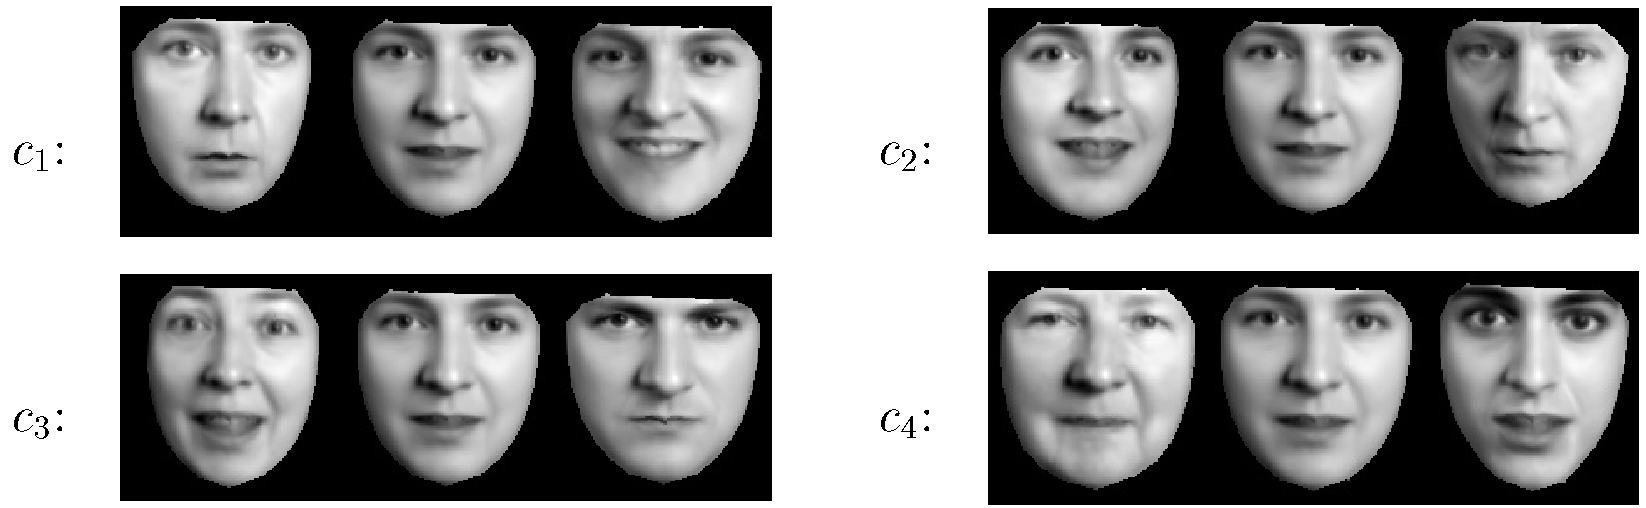
\includegraphics[width=\columnwidth]{ch2/figures/firstfourAAM.jpg}
  \caption{First four modes of appearance variation ($\pm 3$ sd) \cite{Cootes2001}}
  \label{fig:AAMvariation}
 \end{center}
\end{figure} 

\subsubsection{Model Matching}
Assuming a reasonable approximation, the model matching algorithm is to find the parameters of such a model which synthesises an image as close as to a target image. AAM matching is an optimisation problem in which the differences between a new image and a synthesised image by the appearance model is minimised. A different vector $\delta \mathbf{I}$ is defined as the subtracting between the gray-level values in the image and the gray-level values for the current model parameters. To find the best match between image and model, the magnitude of the difference vector $\Delta=|\delta \mathbf{I}|^2$ is minimised by varying with model parameters $\mathbf{c}$. The displacement of each model parameter from the correct value leads a special pattern in  $\delta \mathbf{I}$ and the error in the model parameters  $\delta \mathbf{c}$. In the training stage of AAM, a linear model is applied to learn the relationship between $\delta \mathbf{I}$ and $\delta \mathbf{c}$. In the matching stage of AAM, the knowledge of relationship is applied in an iterative algorithm for minimising $\Delta$. The iterative AAM matching is shown in \mbox{Figure} \ref{fig:AAMmatching}.
\begin{figure}[ht]
 \begin{center}
  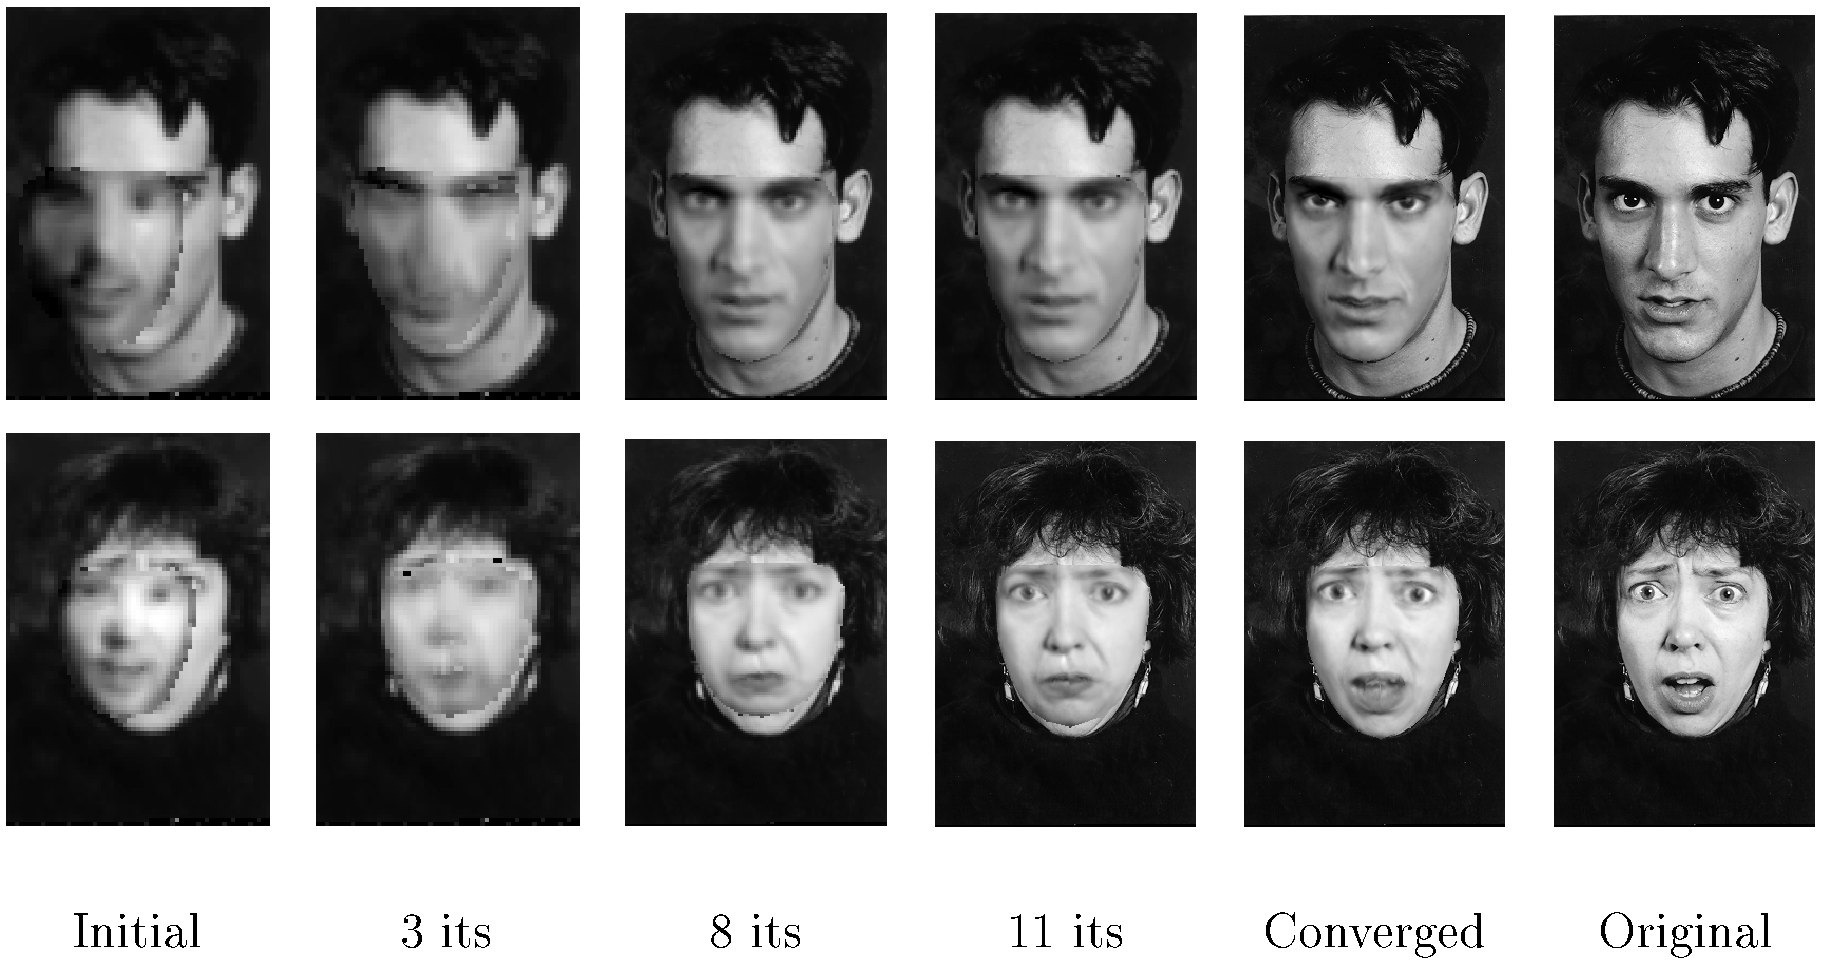
\includegraphics[width=\columnwidth]{ch2/figures/AAMmatching.jpg}
\caption{The two examples of the AAM matching iterations. \cite{Cootes2001}}
\label{fig:AAMmatching}
 \end{center}
\end{figure} 

\subsubsection{Recognition}
Once the appearance model has been matched to a new image, a full set of parameters can be computed. The classification system is used for recognising the individual appearing in an image. The classifier is trained by computing the appearance parameters for all training images (10 images for each of the 30 individuals \cite{Lanitis1997}), and establishing the distribution of appearance parameters for each individual. A discriminant analysis approach is used to enhance the effect of the inter-class variation. The metric is used as the Mahalanobis distance measure.

\subsection{Summary on model-based approaches}
The model-based approaches in face recognition exploit the intrinsic physical relationship with real faces. The physical relationship can be explained in geometric structure. Face variations due to different pose, illumination, and expression are modelled explicitly, which gives the possibility to handle these variations in practice. Prior knowledge on human faces is integrated into the approaches, so that not only statistic rules but also human knowledge are involved in face recognition. However, the model-based approaches suffer some drawbacks. 1) Constructing a model is very complicated and needs a lot of human intervention. Facial feature points are difficult to extract automatically with sufficient robustness. 2) Fitting or matching a model on an image is an optimisation process, which has highly computational costs since it is prone to be trapped into local minima. 3) The recognition results depend heavily on the results of fitting, so that there is a tradeoff between accuracy and computational cost in the fitting process. 4) For matching a model, a high resolution and high quality image is required. The model-based approaches also need complicated initialisation.

\section{3-D Morphable Face Model}\label{sec:3DMM}
The human faces can be treated as a manifold surface in a 3-D space. The 3-D morphable face model (3DMM) for face image synthesis and face recognition is developed by Blanz \textit{et al.} \cite{Blanz1999,Blanz2003}. One advantage of the 3-D morphable face model is that it can easily handle variation on pose and illumination instead of 2-D models, \textit{e.g.}, EBGM and AAM. The variance of pose and illumination is always obstacles for face recognition in 2-D space. Another advantage of the 3-D morphable face model is that a 3-D face surface is extracted from a single 2-D face image, which avoids expensive 3-D face/head scan. Face recognition uses the shape and texture parameters of the model, which represent intrinsic information of faces. 

\subsection{A Morphable Model of 3-D Faces}
In \cite{Blanz2003}, the morphable model is acquired from 3-D scans of 100 males and 100 females, aged between 18 and 45 years. These scans are recorded with a $Cyberwave$ 3030PS laser scanner. The scans represent face shape in cylindrical coordinates relative to a vertical axis centred as for the head. There are $512$ angular steps covering $360$ and $512$ vertical steps at a spacing of $0.615$mm. After the raw scans are obtained, some preprocessing is needed. 
\begin{enumerate}
 \item Holes are filled and spikes are removed on the face surface.
 \item 3-D data are aligned with a 3D-3D Absolute Orientation \cite{Haralick1992}.
 \item Heads are trimmed along the edge of a bathing cap.
 \item Heads are cut vertically behind the ears to remove the back of the head.
 \item Heads are cut horizontally at the neck to remove the shoulders.
\end{enumerate}
After above preprocessing, a modified optic flow method \cite{Horn1981,Bergen1990} is applied to establish dense point-to-point correspondence between a new face and a reference face. The shape and texture vectors of the reference face are
\begin{equation}
 \mathbf{S}_0 = (x_1,y_1,z_1,x_2,\ldots,x_n,y_n,z_n)^T
\end{equation}
\begin{equation}
 \mathbf{T}_0 = (R_1,G_1,B_1,R_2,\ldots,R_n,G_n,B_n)^T
\end{equation}
where the reference face is a triangular mesh with $75,972$ vertices ($n=75972$), $(x_k,y_k,z_k)$ is Cartesian coordinate for each vertex, and $(R_k,G_k,B_k)$ is the colour values from each vertex (and $k=1,\ldots,n$).

The PCA is performed on the set of shape and texture vectors $\mathbf{S}+i$ and $\mathbf{T}_i$ of $m$ example faces. There $m-1$ eigenvectors $\mathbf{s}_1,\mathbf{s}_2,\ldots$ are computed in the shape vectors from PCA by a Singular Value Decomposition (SVD) \cite{Press1992}. The eigenvectors construct an orthogonal basis on the shape vectors 
\begin{equation}
 \mathbf{S} = \bar{\mathbf{s}}+\sum_{i=1}^{m-1}\alpha_i\cdot \mathbf{s}_i
\end{equation}
where $\bar{\mathbf{s}}$ is the average from each shape vector, $\bar{\mathbf{s}}= \frac{1}{m}\sum_{i=1}^m \mathbf{S}_i$. So as to the texture vectors, an orthogonal basis is
\begin{equation}
 \mathbf{T} = \bar{\mathbf{t}}+\sum_{i=1}^{m-1}\beta_i\cdot \mathbf{t}_i
\end{equation}
The model coefficients $\alpha_i$ and $\beta_i$ are used to represent a face in an image.
\subsection{Morphable Model Fitting}
Face image synthesis defines the positions of vertices of the 3-D model with illumination and colour. During the processing of fitting a model with a novel image, not only the shape and texture parameters $\alpha_i$ and $\beta_i$ are optimised, but also the following rendering parameters are optimised. There are $22$ rendering parameters concatenated into a vector $\rho$: pose angles $\phi$, $\theta$, and $\gamma$, 3-D translation $\mathbf{t}_w$, focal length $f$, ambient lighting intensities $L_{r,amb},L_{g,amb},L_{b,amb}$, directed light intensities $L_{r,dir},L_{g,dir},L_{b,dir}$, the angles $\theta_l$ and $\phi_l$ of the directed light, colour contrast $c$, and gains and offsets of colour channels $g_r,g_g,g_b,o_r,o_g,o_b$. In analysis-by-synthesis iterations, the fitting algorithm finds model parameters and rendering parameters, and produces an image as similar as possible to the input image $\mathbf{I}_{input}$ as shown in \mbox{Figure} \ref{fig:modelvsinput}. 
\begin{figure}[t]
 \begin{center}
 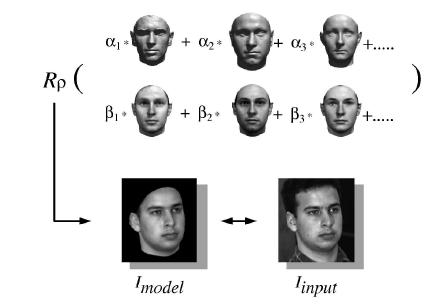
\includegraphics[width=0.77\columnwidth]{ch2/figures/3DMMfitting.jpg} 
 \caption{Fitting a morphable model: analysis by synthesis iterations.\cite{Blanz2003}}
  \label{fig:modelvsinput}
 \end{center}
\end{figure}
The goal of the fitting is to find shape and texture coefficients $\alpha$ and $\beta$ such that rendering $R_{\rho}$ produces an image $\mathbf{I}_{model}$ that is as similar as possible to $\mathbf{I}_{input}$.

The face reconstruction from a single image is shown in \mbox{Figure} \ref{fig:3DMMreconstruction}.
\begin{figure}[ht]
 \begin{center}
  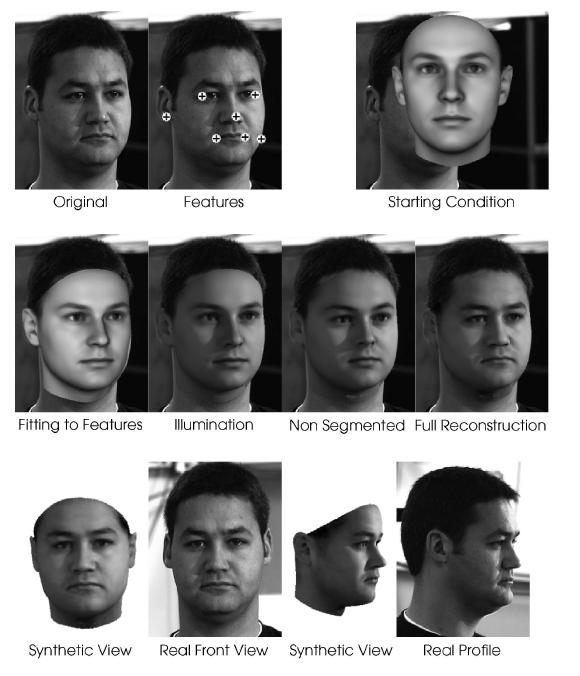
\includegraphics[width=0.77\columnwidth]{ch2/figures/3DMMreconstruction.jpg}
  \caption{The Face reconstruction from a single image by the 3-D morphable model. \cite{Blanz2003}}
  \label{fig:3DMMreconstruction}
 \end{center}
\end{figure}
For initialisation, seven facial feature points, such as the corner of the eyes or the tip of the nose, are marked in image coordinates. On the morphable model, these 7 points are also defined as vertices of the mesh corresponding to the points in the image.
The primary objective in analysing a face is to minimise the sum of square differences over all colour channels and all pixels in the input image and the symmetric reconstruction
\begin{equation}
 E_I = \sum_{x,y}\|  \mathbf{I}_{input}(x,y) -  \mathbf{I}_{model}(x,y) \|^2
\end{equation}
A stochastic version of Newton's method is used to minimise the cost function in the fitting procedure. Because the face model is separated into four regions - eyes, nose, mouth and the surrounding face area, the optimisation is also separated by each region to obtain local parameters, \textit{i.e.}, $\alpha_{r_1}, \beta_{r_1},\ldots,\alpha_{r_4}$ and $\beta_{r_4}$.

\subsection{Recognition}
After fitting the model, recognition can be performed based on model coefficients $\alpha$ and $\beta$, which represent intrinsic shape and texture information of faces. For identification, all gallery images are analysed by the fitting algorithm, and the shape and texture coefficients are stored. Given a probe (testing) image, the fitting algorithm computes coefficients which are compared with all images in the database to find the nearest neighbour. \mbox{Figure} \ref{fig:3DMMrecognition} shows the recognition scheme. Huang \textit{et al.} \cite{Huang2003} extended the 3-D morphable model with component-based recognition. Support Vector Machine (SVM) is used to decompose the face into a set of components. The system achieved $90\%$ recognition rate on a database of $1,200$ real images.
\begin{figure}[t]
 \begin{center}
  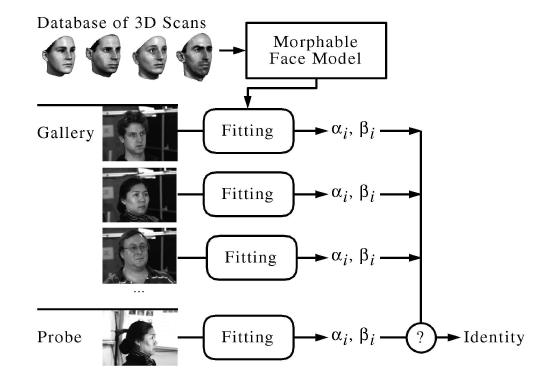
\includegraphics[width=0.77\columnwidth]{ch2/figures/3DMMrecognition.jpg}
  \caption{The recognition scheme in the 3-D morphable model. \cite{Blanz2003}}
  \label{fig:3DMMrecognition}
 \end{center}
\end{figure} 

\section{Other Approaches}
\label{sec:others}
There is a number of other approaches which have been explored in face recognition from different aspects. 
The \textit{trace transform} \cite{Kadyrov2001}, a generalisation of the radon transform, is a new tool for image processing which can be used for recognising faces \cite{Srisuk2003,Srisuk2003EE} under transformations, \textit{e.g.}, rotation, translation and scaling. Hidden Markov Model (HMM) \cite{Nefian1998} is an example of statistical model based approaches for face recognition. The pseudo two-dimensional HMM structure is proposed by Nefian and Hayes \cite{Nefian2000} for face detection and recognition.

\section{Face Database}\label{sec:facedatabase}
Along with the development of face recognition technology, a comparatively large number of face images in both training and testing sets have been collected. The face databases provide researchers a group of well-designed and organised face images, which are used for training and testing. In addition, with the numerous theories and techniques in face recognition, it is clear that evaluation and benchmarking of these algorithms is crucial. The face databases also provide a platform that evaluation could be done.

While there are many databases in use currently, the choice of an appropriate database to be used should be made based on the task given (aging, expressions, lighting etc). Another way is to choose the data set specific to the property to be tested (\textit{e.g.}, how algorithm behaves when given images with lighting changes or images with different facial expressions).

In this section, some face database popularly used by researchers are introduced. An comprehensive review on face databases on face detection, recognition and expression classification is conducted by Gross \cite{Gross2005}.

\subsubsection{Colour FERET}
The FERET \cite{Phillips1996} program set out to establish a large database of facial images that is gathered independently from the algorithm developers. The FERET database is collected in $15$ sessions between August 1993 and July 1996. The database contains $1,564$ sets of images for a total of $14,126$ images that includes $1,199$ individuals and $365$ duplicate sets of images.
A serial of FERET evaluations attract many institutions and companies to participate.
\subsubsection{XM2VTS}
The XM2VTS database \cite{Messer1999} contains four sessions of $295$ subjects taken over a period of four months. Each recording contains a speaking head shot and a rotating head shot. Sets of data taken from this database are available including high quality colour images, $32 KHz$ $16$-bit sound files, video sequences and a 3-D model.
\subsubsection{Yale}
The Yale face database \cite{Georghiades2001} contains $5,760$ single light source images of $10$ subjects each seen under $576$ viewing conditions ($9$ poses by $64$ illumination conditions). For every subject in a particular pose, an image with ambient (background) illumination was also captured.
\subsubsection{PIE}
The PIE database \cite{Sim2003} contains $41,368$ images of $68$ people, each person is under $13$ different poses, $43$ different illumination conditions, and with $4$ different expressions.
\subsubsection{ORL}
The ORL face database \cite{Samaria1994} contains ten different images of each of $40$ distinct subjects. For some subjects, the images were taken at different times, varying the lighting, facial expressions (open or closed eyes, smiling or not smiling) and facial details (glasses or no glasses). All the images were taken against a dark homogeneous background with the subjects in an upright, frontal position (with tolerance for some side movement).
\subsubsection{MIT-CBCL}
The MIT-CBCL face recognition database \cite{Weyrauch2004} contains face images of $10$ subjects. It provides two training sets. The first training set contains high resolution pictures, including frontal, half-profile and profile view. The second training set are synthetic images ($324$ per subject) rendered from 3-D head models of the $10$ subjects. The head models are generated by fitting a morphable model to the high-resolution training images, but the 3-D model is not included in the database. The testing set consists of $200$ images per subject. 
\subsubsection{AR Face Database}
The AR face database \cite{Martinez1998} contains $4,000$ colour images corresponding to $126$ individuals ($70$ men and $56$ women). Images feature frontal view faces with different facial expressions, illumination conditions, and occlusions (sun glasses and scarf).
%\subsubsection{BioID}
%The BioID dataset \cite{Jesorsky2001} consists of $1521$ gray level images with a resolution of $384\times 286$ pixel. Each one shows the frontal view of a face out of $23$ different test persons. For comparison reasons the dataset also contains manually set eye postions.
\subsubsection{UMIST Face Database}
The UMIST face database \cite{Graham1998} consists of $564$ images of $20$ people. Each covering a range of poses from profile to frontal views. Subjects cover a range of race, sex, and appearance. Each subject exists in their own directory labelled and images are numbered consequently as they were taken. The files are all in PGM format, approximately $220 \times 220$ pixels in $256$ shades of grey.
\section{Summary}
In this chapter, an extensive review on face recognition is conducted. Two types of state-of-the-art approaches for face recognition are introduced. A 2-D combined with 3-D approach is also reviewed. Face recognition is still a very challenging topic after 30 years of research \cite{Zhao2003}. Pose and illuminance are still two major problems that degrade the performance of face recognition systems. Appearance-based approaches focus on statistical distribution of facial texture. The texture is locally distributed on human faces. Also, appearance-based approaches abandon some prior information of human faces, \textit{e.g.}, head, hair, ears and so on. Model-based approaches focus on the topologyl and shapes of faces, but ignore the statistical analysis of facial texture. It proves that appearance-based and model-based approaches can be combined, such that appearance-based approaches deal with local texture information, and model-based approaches deal with global shape information.


